\chapter{Experiments And Results}\label{chp:experiments-and-results}
	
%\section{Experiments and Results}
% Ablation studies
% Problem with "global" pose -> incremental pose
% Training
%	- Different learning rate for pretrained flownet
%	- Dropout Regularization
	This chapter presents all experiments conducted on the deep learning model that was introduced in chapter~\ref{chp:the_model}.
	The results shown here give useful insights that supplement the work of \cite{wang2017deepvo}.
	
	\section{Dataset Size and Dropout}
		We start by training the proposed model on the KITTI dataset on small subsequences of 25 frames. 
		Initially, the sequences are divided without overlap, that is, each video frame is part of exactly one subsequence.
		In addition, to simulate a dataset with more subsequences, the overlap is set to 20 frames (80\%). 
		This means that for each subsequence there is another one that differs by 5 frames.
		Table~\ref{tbl:kitti-overlap-and-dropout} compares the test error for models trained with and without overlap.
		\begin{table}[tb]
			\small
			\begin{center}
				\begin{tabular}{ccccrrr}
					\toprule
					\multicolumn{3}{c}{\textbf{Experiments}}	&	& \multicolumn{3}{c}{\textbf{Test error}} 		\\
					\cmidrule(lr){1-3} 					\cmidrule(lr){5-7}
					Length 			& Overlap 	& Dropout	&	& Total 	& Rotation	& Translation	\\ 
					\midrule
					25				& 0			& 0			& 	& 19.0293	& 0.4981	& 18.5312		\\ 
					25				& 20		& 0			&	& 16.5471	& 0.3913	& 16.1558		\\ 
					100				& 20		& 0			&	& 529.9459	& 39.8967	& 490.0493		\\ 
					100				& 80		& 0			& 	& 313.1278	& 47.8437	& 265.2841		\\ 
					100 			& 5			& 0.5		&	& 376.7666	& 43.1578	& 333.6088		\\ 
					%$20\rightarrow120$ 	& 5		& 0.5		&	& 303.7696	& 39.4114	& 264.3582		\\
					$20\rightarrow100$ 	& 5		& 0.5		&	& 289.8579 	& 42.0427 	& 247.8152 		\\
					\bottomrule
				\end{tabular}
			\end{center}
			\caption[Experiments on KITTI: Overlap and dropout]
					{Experiments on KITTI: Overlap and dropout. 
					 Shown is the test error on sequence 10 for different overlap and dropout during training.
					 The evaluation on the test set is performed on sequences of the same size as seen during training, and without overlap.
					 In the last row, the sequence length grows by one frame every epoch.
					 Each model was trained with default parameters for 100 epochs, except the last one which was trained for only 80 epochs.
					 \label{tbl:kitti-overlap-and-dropout}}
		\end{table}
		After the same number of epochs, the test error is about 13\% lower for the model trained on overlapping sequences with a decrease of 21\% for rotation and 12\% for translation.
		The same experiment is repeated by training on sequences of 100 frames with overlap 20 vs. overlap 80. 
		% Total error decreases by about 40\%.
		The translation error decreases by almost 46\%, however, the rotation loss increases.
		A similar observation can be made when using dropout on the LSTM output (before the fully-connected layer), as seen in the second last row of table~\ref{tbl:kitti-overlap-and-dropout}.
		
		For the last experiment in table~\ref{tbl:kitti-overlap-and-dropout}, the sequence length grows by an increment of one frame every epoch, starting from 20 frames and stopping at 100 frames after 80 epochs.
		As we can see, this method of training in combination with the dropout gives the best overall loss on the test set.
		A possible explanation for this could be the that the learning process is faster for short sequences because the LSTM requires a less complex memory mapping in order to remember the coordinate transforms from earlier time steps, including the first one.
		A gradual refinement of such a mapping may be less challenging for the optimization as opposed to learning it directly from long sequences.
		\todo{Need more explanation here.}
		
		Although the numbers in the table can be used to compare the different experiments, they are not very insightful by themselves.
		From the sum of squared differences alone, it is not possible to understand how the error behaves across the sequence.
		For better visualization, we can compute the error at regular distance intervals along the estimated path.
		Figure~\ref{fig:kitti-avg-rotation-translation-error-vs-path-distance} shows translation and rotation errors for path distance on subsequences of the KITTI sequence 10.
		\begin{figure}
			\centering
			\includegraphics[width=0.7\linewidth]{Python-Plots/deepvo-KITTI/relative-rotation-and-translation-error-along-path-overlap80}
			\caption[Experiments on KITTI: Average rotation- and translation error vs. path distance]
					{Experiments on KITTI: Average rotation- and translation error vs. path distance.
					 The relative rotation- and translation error is evaluated at equal intervals along the subsequences of KITTI sequence 10.
					 The errors at the same distance are averaged over all sequences of that length.
					 \label{fig:kitti-avg-rotation-translation-error-vs-path-distance}}
		\end{figure}
		The relative rotation error is the angle of rotation around the axis corresponding to the relative rotation between estimated and ground truth pose.
		\todo{refer to equations introduced in previous chapter}
		
		\paragraph{Conclusion}
		From these experiments, we can conclude that sequence overlap and dropout have a positive impact on the generalization of translation estimates.
		Especially when training data is scarce, the overlap method can be utilized to artificially increase the dataset and reduce the error on the test data.
		
	\section{The Problem on Long Sequences}
		Ideally, we would like to train the model on sequences with an arbitrary number of frames.
		Due to the high cost of backpropagation in RNNs, the number of frames that can be processed at a time is limited by the available memory.
		However, testing the model is very fast because only the forward operation is performed.
		In the experiments before, the model was always tested on subsequences with the same length as during training.
		
		\begin{table}[tb]
			\small
			\begin{center}
				\begin{tabular}{cccrrr}
					\toprule
					\multicolumn{2}{c}{\textbf{\#Frames}}	&	& \multicolumn{3}{c}{\textbf{Test error}} \\ 
					\cmidrule(lr){1-2} 									\cmidrule(lr){4-6}
					Training 		& Test 			&	& Total 	& Rotation	& Translation	\\ 
					\midrule
					25				& 25			&	& 16.5471	& 0.3913	& 16.1558		\\
					25				& 100			&	& 1060.7528	& 37.6196	& 1023.1332		\\
					100				& 100			&	& 529.9459	& 39.8967	& 490.0493		\\ 
					\bottomrule
				\end{tabular}
			\end{center}
			\caption[Experiments on KITTI: Testing on longer sequences]
					{Experiments on KITTI: Testing on longer sequences. 
					 When testing on sequences with more frames, the error becomes extremely high compared to the model trained on 100 frames.
				 \label{tbl:kitti-testing-on-longer-sequences}}
		\end{table}

		\begin{figure}
			\centering
			\begin{subfigure}[b]{0.5\linewidth}
				\centering
				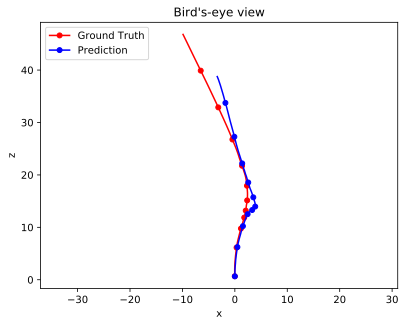
\includegraphics[width=\linewidth]{Experiments/trained-on-25-frames}
				\caption{
					\label{fig:0}
				}
			\end{subfigure}%
			\begin{subfigure}[b]{0.5\linewidth}
				\centering
				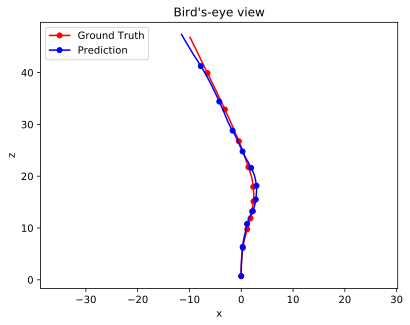
\includegraphics[width=\linewidth]{Experiments/trained-on-100-frames}
				\caption{
					\label{fig:1}
				}
			\end{subfigure}%
			\caption[Training and testing on different sequence length]
					{Training and testing on different sequence length. 
				 Two models tested on a KITTI subsequence of 100 frames and trained on sequences of (a) 25 frames and (b) 100 frames. 
				 The markers in the plot are shown every ten frames.
				 The scale of the axes is in meters.
				 \label{fig:kitti-testing-on-longer-sequences}}
		\end{figure}


	\section{Training with Incremental Poses}
		
		\begin{table}[tb]
			\small
			\begin{center}
				\begin{tabular}{cccccrrr}
					\toprule
					\multicolumn{5}{c}{\textbf{Experiments}}		& \multicolumn{3}{c}{\textbf{Test error}} 		\\
					\cmidrule(lr){1-4} 	\cmidrule(lr){6-8}
					\multicolumn{2}{c}{Length} & Dropout & LSTM &	& Total & Rotation & Translation	\\ 
					Training & Test & & & & & & \\
					\midrule
					25 & 25		& 0			& \xmark 	& 	& 22.4305	& 0.5121	& 21.9184		\\ 
					25 & 100	& 0			& \xmark 	& 	& 378.8834	& 48.4604	& 330.4230 		\\ 
					25 & 25		& 0			& \cmark 	& 	& 22.0498	& 0.5642	& 21.4856 		\\ 
					25 & 100	& 0			& \cmark 	& 	& 335.5754	& 16.5476	& 319.0277 		\\ 
					25 & 25		& 0.5		& \cmark 	& 	& 21.0171	& 0.4957	& 20.5214		\\ 
					25 & 100	& 0.5		& \cmark 	& 	& 301.5090	& 22.9736	& 278.5354 		\\ 
					\bottomrule
				\end{tabular}
			\end{center}
			\caption[Experiments on KITTI: Replacing the LSTM with an affine layer]
					{Experiments on KITTI: Replacing the LSTM with a fully-connected layer.
					 \label{tbl:kitti-removing-lstm}}
		\end{table}
		
		\begin{figure}
			\centering
			\begin{subfigure}[b]{0.5\linewidth}
				\centering
				\includegraphics[width=\linewidth]{Python-Plots/deepvo-KITTI/rotation-error-per-meter-comparison-Dropout-No-LSTM}
				\caption{
					Rotation
					\label{fig:avg-rotation-error-dropout-no-LSTM}
				}
			\end{subfigure}%
			\begin{subfigure}[b]{0.5\linewidth}
				\centering
				\includegraphics[width=\linewidth]{Python-Plots/deepvo-KITTI/translation-error-per-meter-comparison-Dropout-No-LSTM}
				\caption{
					Translation
					\label{fig:avg-translation-error-dropout-no-LSTM}
				}
			\end{subfigure}%
			\caption[Average rotation- and translation error]
					{\label{fig:avg-rotation-and-translation-error-dropout-no-LSTM}}
		\end{figure}
		
		\begin{table}[tb]
			\small
			\begin{center}
				\begin{tabular}{lcrrrr}
					\toprule
					%\multicolumn{2}{c}{\textbf{Experiments}}		& \multicolumn{4}{c}{\textbf{Test error}} 		\\
					%\cmidrule(lr){1-2} 	\cmidrule(lr){3-6}
					\textbf{Hidden state} & & \multicolumn{2}{c}{\textbf{Relative Pose}} & \multicolumn{2}{c}{\textbf{Global Pose}} \\
					& & Rotation & Translation & Rotation & Translation \\
					\midrule
					Reset 		& 			& 0.2319	& 5.7220	& 9.8600	& 262.7984		\\ 
					Keep		&			& 0.3097	& 8.5461	& 12.7551	& 426.7877		\\
					\bottomrule
				\end{tabular}
			\end{center}
			\caption[Experiments on VIPER: Carrying over the hidden state vs. resetting it]
					{Experiments on VIPER: Carrying over the hidden state vs. resetting it.
					 \label{tbl:kitti-removing-lstm}}
		\end{table}
	
		\begin{figure}
			\centering
			\includegraphics[width=\linewidth]{example-image-a}
			\caption{Convergence speed comparison state reset vs. keep.}
		\end{figure}
		
		\subsection{Euler Angles}
		
		\subsection{Quaternions}

		\begin{figure}
			\centering
			\begin{subfigure}[b]{\linewidth}
				\centering
				\includegraphics[width=0.45\linewidth]{example-image-a}
				\includegraphics[width=0.45\linewidth]{example-image-a}
				\caption{
					Long, curve
					\label{fig:0}
				}
			\end{subfigure}%
			\\
			\begin{subfigure}[b]{\linewidth}
				\centering
				\includegraphics[width=0.45\linewidth]{example-image-b}
				\includegraphics[width=0.45\linewidth]{example-image-b}
				\caption{
					Short
					\label{fig:0}
				}
			\end{subfigure}%
			\\
			\begin{subfigure}[b]{\linewidth}
				\centering
				\includegraphics[width=0.45\linewidth]{example-image-c}
				\includegraphics[width=0.45\linewidth]{example-image-c}
				\caption{
					\label{fig:0}
				}
			\end{subfigure}%
			\caption[Qualitative results for motion estimation on KITTI]
					{Qualitative results for motion estimation on KITTI.
				 Left column: Visualization of the estimated and true path.
				 Right column: Plot of each coordinate axis.
				 Markers are shown for every \todo{xx} frames.
					\label{fig:0}}
		\end{figure}


		\begin{figure}
			\centering
			\begin{subfigure}[b]{\linewidth}
				\centering
				\includegraphics[width=0.45\linewidth]{example-image-a}
				\includegraphics[width=0.45\linewidth]{example-image-a}
				\caption{
					Long, curve
					\label{fig:0}
				}
			\end{subfigure}%
			\\
			\begin{subfigure}[b]{\linewidth}
				\centering
				\includegraphics[width=0.45\linewidth]{example-image-b}
				\includegraphics[width=0.45\linewidth]{example-image-b}
				\caption{
					Short
					\label{fig:0}
				}
			\end{subfigure}%
			\\
			\begin{subfigure}[b]{\linewidth}
				\centering
				\includegraphics[width=0.45\linewidth]{example-image-c}
				\includegraphics[width=0.45\linewidth]{example-image-c}
				\caption{
					\label{fig:0}
				}
			\end{subfigure}%
			\caption[Qualitative results for motion estimation on VIPER]
					{Qualitative results for motion estimation on VIPER.
				 \label{fig:0}}
		\end{figure}